%%%%%%%%%%%%%%%%%%%%%
% Analysis and Results %
%%%%%%%%%%%%%%%%%%%%%

This thesis aims to analyze the relationships between different road networks and road network similarity methods. In particular,  (1) the similarities between different road networks are determined, (2) determine the correlations between the different network similarity methods used for identifying the similarities between the different road networks, (3) cluster road networks that are similar, and (4) cluster methods that are similar. Figure's 4.1 and 4.2 contains an overview of the process respectively. The problem is explicitly approached through the use of network-similarity ranking. A reference network Gr and a collection of comparison networks H1, H2,...., Hk are given with this application. The similarity between Gr and each Hi is calculated using a network-similarity method, and the comparison networks are ranked in order of their similarity to the reference network Gr. Similar methods that generate similar scores can be compared over a wide range of values by approaching the problem from the standpoint of ranking rather than raw similarity scores. Given a reference network, a collection of networks to be compared, and m network similarity methods, M rankings of the comparison networks are generated. The m rankings are then compared to determine the degree of similarity between the different methods.
 To find road networks with similar structures and patterns, the road networks are clustered.
The complete-linkage hierarchical clustering method is used for this step because it produces a dendrogram with many small clusters, which provides insight into which road network groups are closely similar or correlated. The clustering results show which groups of road networks have comparable similarities in their structure and pattern. To find methods with similar behavior, we implement the same approach as used earlier to find similar road networks; the difference is that the methods are clustered based on pairwise Kendall-Tau distances, which is then followed by a complete-linkage hierarchical clustering because it produces a dendrogram with many small clusters, which provides insight into which groups of methods are closely correlated—the results of this clustering show which groups of methods have similar behavior.

\begin{figure}[h]
\centering
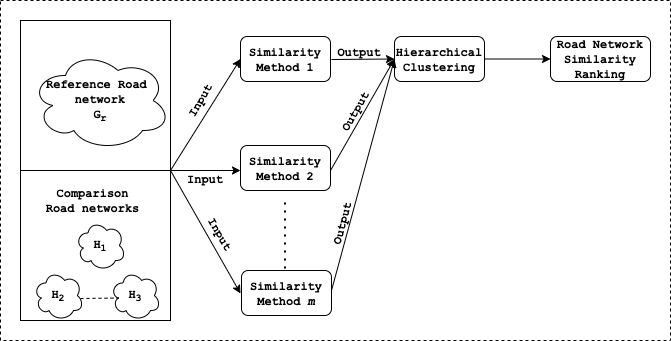
\includegraphics[width=1.25\textwidth,center]{picture/network_ranking.png}
\caption[Miniaturtrichter]{Road Networking Similarity and Ranking}
\label{fig:network ranking}
\end{figure}

\subsection{Grid Road Network Similarity Analysis}
\subsection{Radial Road Network Similarity Analysis}
\subsection{Tree Road Network Similarity Analysis}
\subsection{Linear Road Network Similarity Analysis}
\subsection{Cul de Sac Road Network Similarity Analysis}
